\subsection{综合指标变化过程}\label{ch4:sec:process}

\begin{figure*}[ht!]
	\centering
	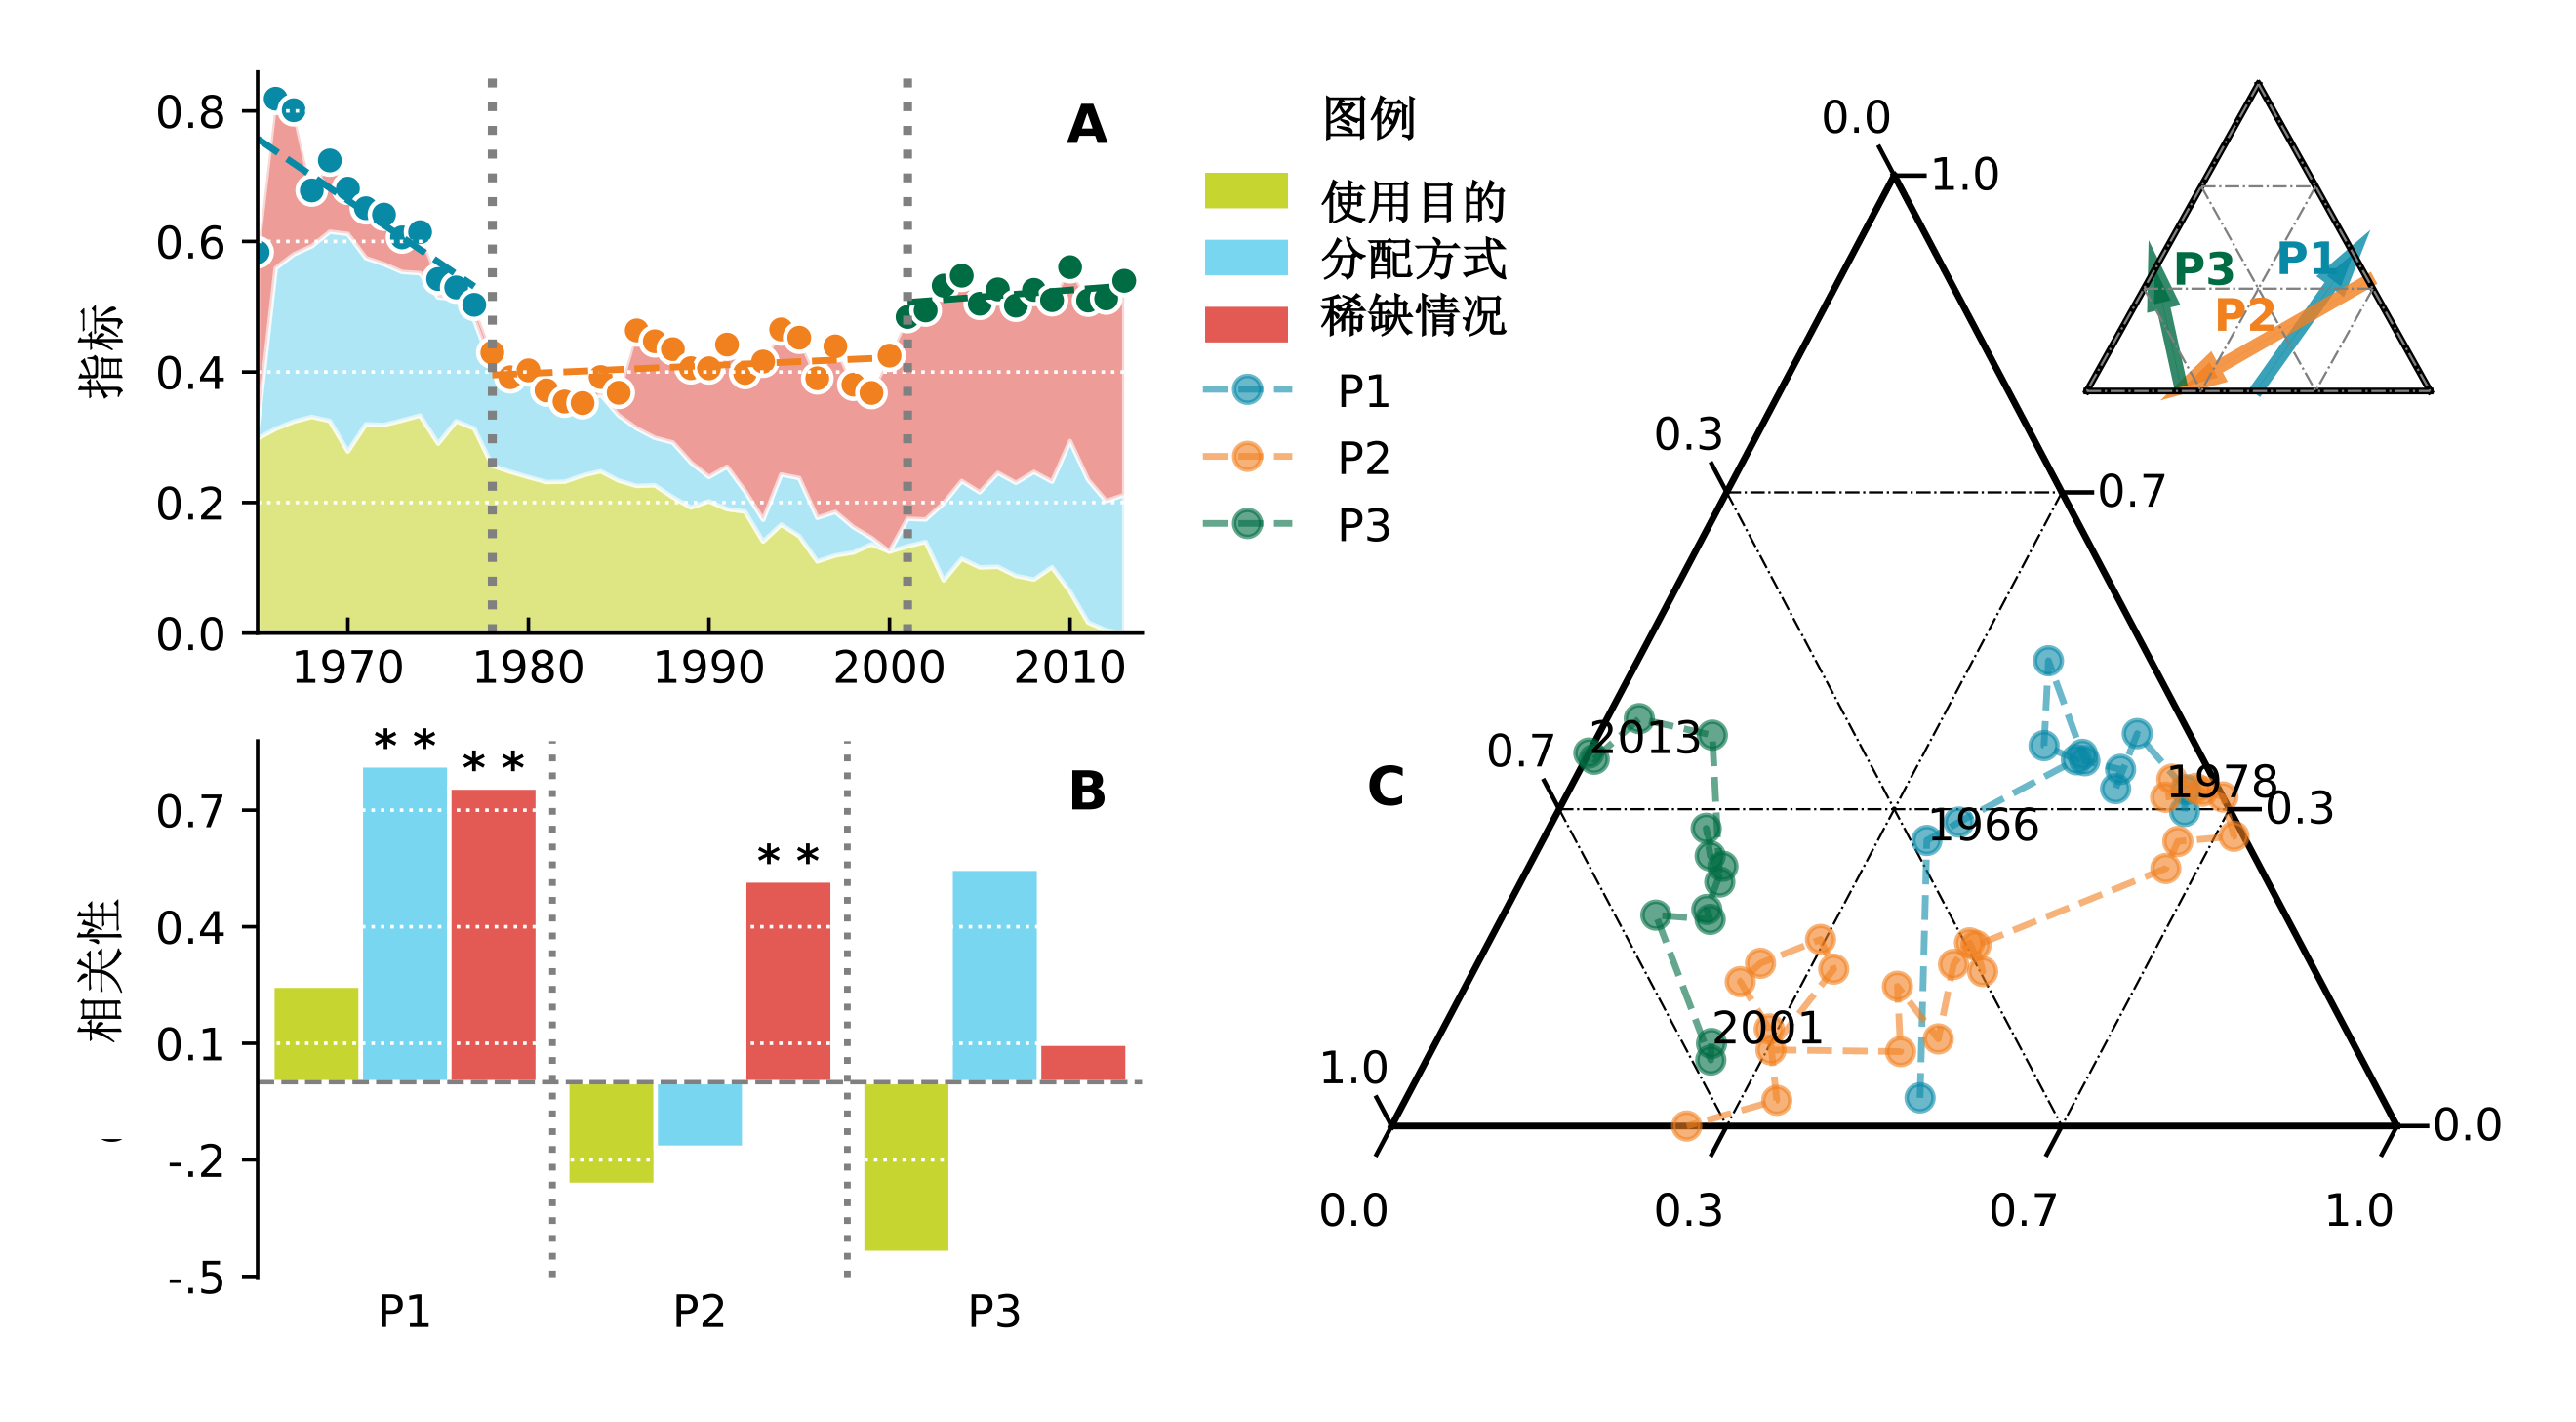
\includegraphics[width=\textwidth]{img/ch4/ch4_index.png}
	\caption[IWGI指数反映黄河流域的水治理变化阶段]{IWGI指数反映黄河流域的水治理变化阶段。两个突变点将1965年以来的黄河流域水治理划分为三个阶段,第一阶段(P1): 1965 \textendash{} 1978年,第二阶段(P2): 1979 \textendash{} 2001年,第三阶段(P3): 2002 \textendash{} 2013年。
	\textbf{A} 检测IWGI的突变点和三个指标的各自贡献:“稀缺情况(S)”、“使用目的(P)”和“分配方式(A)”。1978年和2001年出现了两个显著的变化点($p<0.01$)。
	\textbf{B}  各阶段的IWGI变化与三个指标各自变化的相关性。
	\textbf{C} IWGI随时间变化的同时,三个指标贡献比例的组合不断改变,致使水治理向不同方向发生阶段性转移。
	}\label{ch4:fig:IWGI}
\end{figure*}

IWGI在研究时段内存在两个突变点,将1965年以来的黄河流域水治理划分为三个阶段,第一阶段(P1): 1965 \textendash{} 1978年,第二阶段(P2): 1979 \textendash{} 2001年,第三阶段(P3): 2002 \textendash{} 2013年,而“稀缺情况(S)”、“使用目的(P)”和“分配方式(A)”的三个指标在每个阶段的贡献不同(图~\ref{ch4:fig:IWGI}A)。
% 第一阶段
在第一个时期(P1, 1965 \textendash{} 1978年)水资源压力对IWGI的贡献很小,“使用目的”和“分配方式”的指标的贡献更大(平均分别为$49.45\%$和$34.95\%$),但均呈现出显著的下降趋势($p<0.01$,图~\ref{ch4:fig:IWGI}~B),导致此时期IWGI迅速下降。
% 第二阶段
在第二阶段(P2, 1979 \textendash{} 2001年),水资源压力指标的显著增加($p<0.01$)并为IWGI的略微上升做出主要贡献($p<0.01$,图~\ref{ch4:fig:IWGI}~A),而“使用目的”和“分配方式”的指标对IWGI的变化起了消极作用。
% 第三阶段
最后,在第三个时期(P3, 1995 \textendash{} 2013),尽管水资源压力指标在贡献中保持着$57.11\%$的最突出份额,但其数值已几乎保持不变,反而是“使用目的”的指标的降低和“分配方式”指标的增加,共同推动了综合指标IWGI的变化。
%的整体
综上所述,“稀缺情况(S)”、“使用目的(P)”和“分配方式(A)”的三个指标在不同时期对黄河流域水治理整体特征变化的贡献不同,将其演变历史划分为明显的三个阶段,依据其各自特点可命名为:集中供水时期、治理转变时期、适应增强时期(对应时间阶段分别为1965 \textendash{} 1978年、1979 \textendash{} 2001年、2002 \textendash{} 2013年(图~\ref{ch4:fig:IWGI}~C)。

\subsection{各子指标变化}

\begin{figure}[!ht]
  \centering
  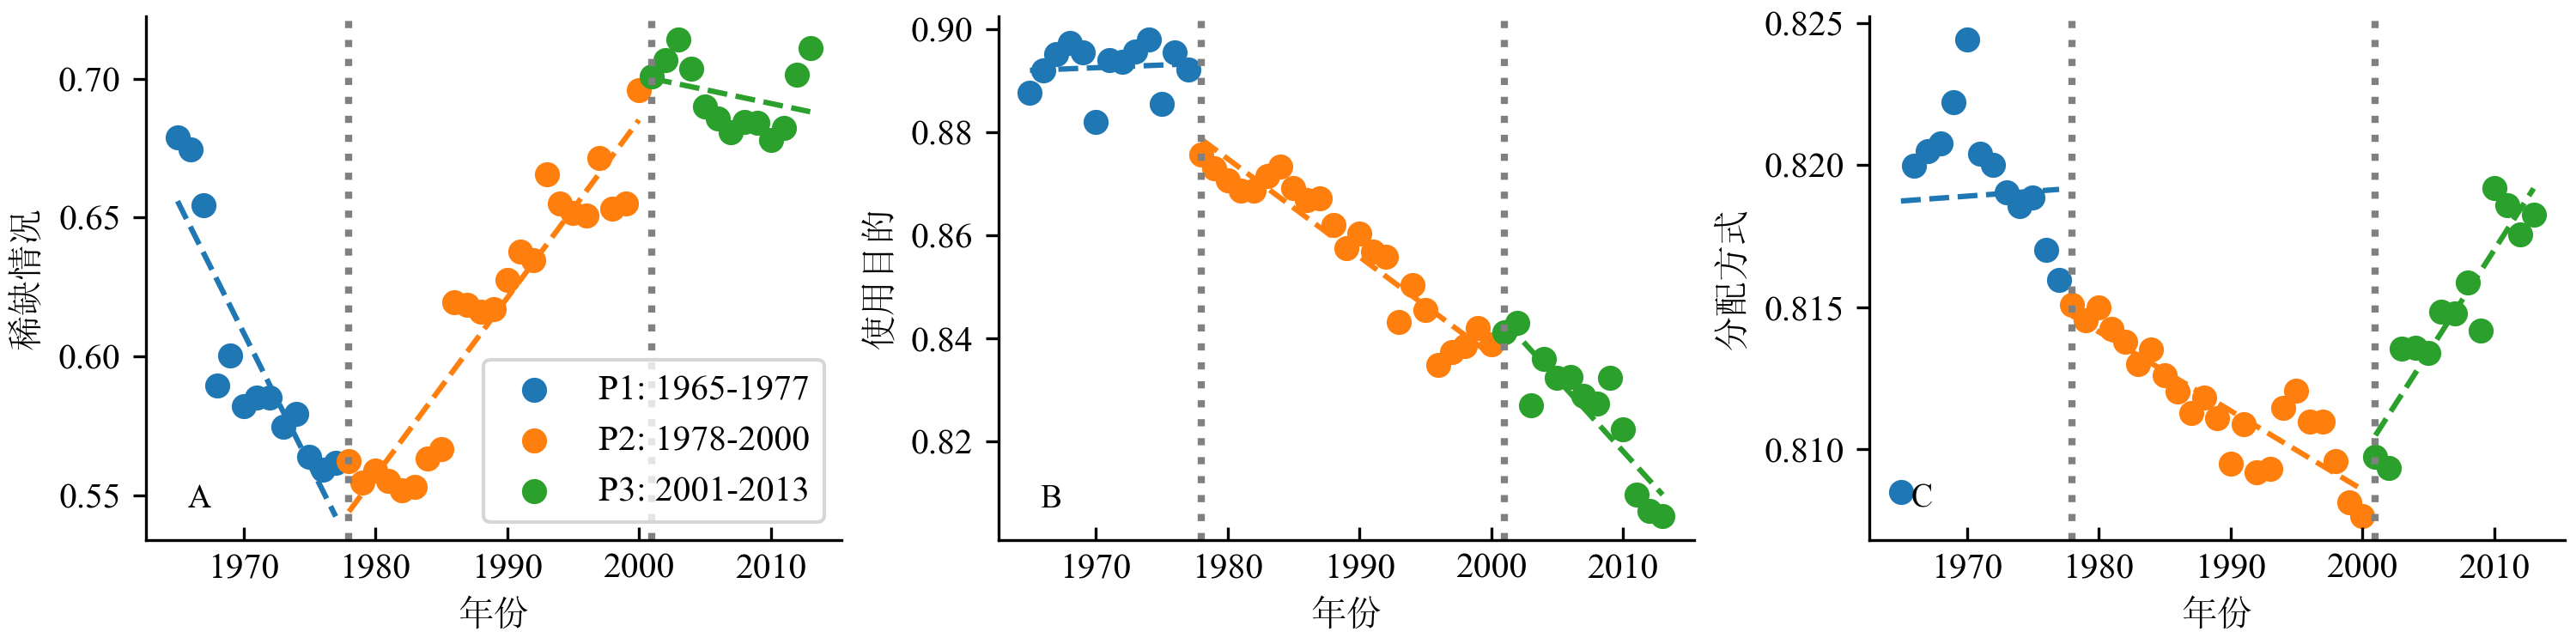
\includegraphics[width=\textwidth]{img/ch4/ch4_indicators.png}
  \caption[各子指标变化趋势]{
	各子指标变化趋势。
	\textbf{A} 稀缺情况(S)
	\textbf{B} 使用目的(P)
	\textbf{C} 分配方式(A)
}\label{ch4:fig:indicators}
\end{figure}


构成稀缺情况的指标(SFV指数)在研究时段(包括三个不同时期)内呈现出先降低、然后迅速增加、最后再次略微降低的变化趋势(图~\ref{ch4:fig:indicators}~A)。
% ,表明水资源压力先减少再迅速增加,后趋于稳定
源区、上游、中游、下游这四个不同的区域中(表~\ref{ch4:tab:sfv_contribution}),源区对三个时段的SFV指标变化几乎没有贡献,下游也仅在治理转变时期和适应增强时期呈现微弱的负向贡献。
对稀缺情况影响最大的是黄河的上游和中游,上游在集中供水时期和治理转变时期都是SFV变化的最大贡献区域,中游则在适应增强时期做出最大贡献。

% Table generated by Excel2LaTeX from sheet 'sfv各区域贡献'
\begin{table}[!ht]
  \centering
  \caption{黄河源区、上中下游对稀缺情况指标(IS)变化的贡献}
    \begin{tabularx}{0.5\textwidth}{lrrr}
    \toprule
          & \multicolumn{1}{l}{$1966-1978$} & \multicolumn{1}{l}{$1978-2001$} & \multicolumn{1}{l}{$2001-2013$} \\
    \midrule
    源区 & 0.00\% & 0.00\% & 0.00\% \\
    上游 & 90.95\% & 89.94\% & -5.28\% \\
    中游 & 9.05\% & 36.42\% & 123.86\% \\
    下游 & 0.00\% & -26.36\% & -18.58\% \\
    \bottomrule
    \end{tabularx}%
  \label{ch4:tab:sfv_contribution}%
\end{table}%


在用水目的上,供给性用水比例在集中供水时期基本保持不变,但在治理转变时期和适应增强时期呈现迅速下降的趋势(图~\ref{ch4:fig:indicators}~B)。
三个时段都是由灌溉用水的变化主导了该比例变化,城市、农村的人居用水、农村牲畜用水等几乎对该比例的变化没有影响(表~\ref{ch4:tab:ip_contribution})。

% Table generated by Excel2LaTeX from sheet 'purpose各区域贡献'
\begin{table}[!ht]
    \centering
    \caption{不同用水部门对使用目的指标(IP)变化的贡献}
      \begin{tabularx}{0.75\textwidth}{lrrr}
      \toprule
            & \multicolumn{1}{l}{P1: $1965-1977$} & \multicolumn{1}{l}{P2: $1978-2000$} & \multicolumn{1}{l}{P3: $2001-2013$} \\
      \midrule
      IP总变化 & 0.45\% & -3.68\% & -3.57\% \\
      灌溉用水   & 45.02\% & 13.59\% & -6.11\% \\
      城市居民用水 & 1.03\% & 0.53\% & -0.61\% \\
      农村居民用水 & 1.86\% & 0.61\% & -0.37\% \\
      农村牲畜用水 & 0.48\% & 0.20\% & -0.16\% \\
      \bottomrule
      \end{tabularx}%
    \label{ch4:tab:ip_contribution}%
  \end{table}%
  

分配方式的指标变化呈现明显“V形”趋势,表明黄河的源区、上游、中游、下游之间水资源呈现先逐渐远离均匀分配,又在2000年后逐渐趋于平均的变化过程(图\ref{ch4:fig:indicators}~C)。
